\section{At many times, the conditional transition probabilities do not change}

For $\lambda$-almost every $\xi \in X$ one can consider the conditional probability measure $\P^{\xi}$, so that one has $\P=\int_{X}\P^{\xi}d\lambda(\xi)$. 
These measures are Markov and determine homogeneous (in time, not space) Markov chains on $G$ with transition probabilities
\[
\P^{\xi}\left[ w_{n+1}=g\mid w_n=h \right] =\P\left[ w_{n+1}=g\mid w_n=h\right] \frac{dg_{*}\lambda}{dh_{*}\lambda}(\xi)=\mu(h^{-1}g)\frac{dg_{*}\lambda}{dh_{*}\lambda}(\xi),
\]
for each $g,h\in G.$ 
(This is easy to see. For a reference, look at Lemma 14.33 on page 490 in the book of Lyons-Peres)
The following Lemma implies that the probability of multiplying by $a \in G$ in the conditional random walk is $\mu(a)$ whenever $w_n = g$ and the limit point $\xi \notin g I$.

\begin{lemma}\label{lem: invariant Radon nykodym derivative}
 For every $g\in G$ and $\lambda$-almost every $\xi \notin g I$ we have
	\[
	\frac{d(ga)_{*}\lambda}{dg_{*}\lambda}(\xi)=1.
	\] 
\end{lemma}
\begin{proof}
    Indeed, let $A\subseteq \mathbb{S}^1\setminus g(I)$ be any measurable subset with $\lambda(A)>0$ and $\xi \in A$. Then
    $$ g_{*}\lambda(A) =\lambda(g^{-1}A) =\P\left[ \xi(\mathbf{w})\in g^{-1}A\right] = \P\left[ \xi(\mathbf{w})\in (ga)^{-1}A\right] 
    =(ga)_{*}\lambda(A).$$
    The third step follows from the fact that $a^{-1} g^{-1}A = g^{-1}A$ which follows from $g^{-1}A \subset \mathbb{S}^1\setminus I$, that is, $A \subset \mathbb{S}^1\setminus g(I)$.
\end{proof}

Next, we wish to estimate the number of times $n$ for which $w_n^{-1} \xi \notin I$.

\begin{proposition}[Equidistribution]\label{prop:equidistributionXi}
For $\nu$-almost every $\xi \in S^1$, for $\P^\xi$-almost every $\mathbf{w} = \{w_n\}_{n \in \N} \in G^\N$ the convergence of probability measures
\[
\frac{1}{n}\sum_{k = 0}^n 1_{w_n^{-1}(\xi)} \xrightarrow[n \to \infty]{} \nu
\]holds in the weak-$\ast$ topology.
\end{proposition}
\begin{proof}
    \cite[Proposition 4.9]{Malicet2017} shows that for any $x \in S^1$, $\P$-almost surely the convergence
    \begin{equation}\label{eq:equidistributionP}
    \frac{1}{n}\sum_{k = 0}^n 1_{w_n^{-1}(x)} \xrightarrow[n \to \infty]{} \nu
     \end{equation} holds in the weak-$\ast$ topology. We conclude that for $\nu$-almost all $\xi$, \eqref{eq:equidistributionP} holds $\P^\xi$-almost surely.

Fix an arbitrary $x \in S^1$. Recall that we denote $\xi \colon (G^\N, \P) \to (S^1, \nu)$ the boundary map that arises from the action of $G$ on the circle.

Theorem \ref{thm:mean} shows that there exists $\lambda > 0$ such that
\[
\E \left[ d\left(w_n^{-1}(x), w_n^{-1}(\xi(\mathbf{w})) \right) \right] \leq  e^{-\lambda n}
\] for all $n \in \N$, so in particular the sum
\[
\sum_{n \geq 0} d\left(w_n^{-1}(x), w_n^{-1}(\xi(\mathbf{w})) \right)
\] is finite $\P$-almost surely. Thus for $\nu$-almost every $\xi$, the sum 
\[
\sum_{n \geq 0}d(w_n^{-1}(x), w_n^{-1}(\xi) )
\] is finite $\P^\xi$-almost surely. This condition coupled with \eqref{eq:equidistributionP} gives the conclusion.
\end{proof}

\begin{corollary}\label{prop:typeIII}
    For $\nu$-almost every $\xi \in S^1 \setminus I$ there exists $N \in \N$ such that for all $n \geq N$,
    \[
    \E^\xi \left[\, \abs{0 \leq k \leq n \mid  \xi \in w_k I } \,\right] \leq 2 \nu(I) n.
    \]
\end{corollary}
\begin{proof}
    The statement follows from the equality
    \[
    \E^\xi\left[\, \abs{0 \leq k \leq n \mid  \xi \in w_k I }\,\right] = \sum_{k = 0}^n \P^\xi\left[ w_n^{-1}(\xi) \in I\right]
    \]and the equidistribution of $\{w_n^{-1}(\xi)\}_{n \in \N}$ from Proposition \ref{prop:equidistributionXi}.
\end{proof}

Conclude that for a dense subset of the times, the conditional transition probabilities are identical to the unconditional ones.

\section{The lower bound on the relative entropy and proof of Theorem \ref{thm:entropy}}
\textbf{QUESTION:} So we pick up an element $a$ whose support $I$ has arbitrarily small measure $\nu(I)$, and find $n_0$ sufficiently high such that $\mu^{* n_0}(a)>0$.
Why do we know such an $a$ exists??
Is this some structural result about proximal subgroups?

We saw that there exists $0<c<1$ such that $\E Z_n \geq c n$.
Pick $a$ such that $\nu(I) \leq c/8$

We recall the following basic fact about random variables, which is pigeonholing in disguise.
Let $0 \leq X \leq 1$ be a real-valued random variable with mean $\E[X] > \lambda > 0$.
Then
$$\P( X > \lambda/2) \geq \lambda/2.$$
(Why? We have $\lambda < \E[X] \leq \lambda/2 \P( X \leq \lambda/2) + 1 \P( X > \lambda/2) \leq \lambda/2 + \P( X > \lambda/2)$.)

%Recall the random variable $Z_n$ which is the maximum number of disjoint subintervals.
%We saw that $\E_{\xi} \E[Z_n|\xi] = \E Z_n \gtrsim c n$ for some $c>0$.
Fix $\xi \in \mathbb{S}^1$ and consider the random variable $0 < \frac{Z_n|\xi}{n} \leq 1$.
We have
$$\P^\xi\left( \frac{Z_n}{n} > \frac{\E[Z_n|\xi]}{2n}\right) \geq \frac{\E[Z_n|\xi]}{2n}.$$
Consider the set of infinite trajectories $\boldsymbol{w}$ with limit point $\xi$ and $Z_n > \E[Z_n|\xi]/2$.
To each such trajectory $\boldsymbol{w}$ we fix a set $I = \{i_1,...,i_k\} \subset [n]$ of $k = \lceil \E[Z_n|\xi]/2\rceil$-many times such that the intervals 
$\{w_{i_1}I,...,w_{i_k}I\}$ are disjoint
and such that $w_{i_j+1}w_{i_j}^{-1} \in \{1,a\}$ for each $j=1,..,k$.
We assign this trajectory to the collection $q$ consisting of times $i_1+1,...,i_k+1$ along with all the jumps in the remaining $n-k$ times.
Denote the set of all such collections by $A_{n,\xi}$.
By construction,
$$\P^\xi\left[ \cup_{q \in A_{n,\xi}} T^{a,1}(q)\right] \geq \frac{\E[Z_n|\xi]}{2n}.$$
Also, as noted in the preliminary section, each $T^{a,1}(q)$ is satisfactory (that is, any two distince trajectories in $T^{a,1}(q)$ end up at two distinct elements at time $n$).

%Consider the set of all $\xi$ such that
%$$\dfrac{\E[Z_n|\xi]}{n} \geq 2 \nu(I).$$
Because we chose $a$ such that $\nu(I)$ is sufficiently small, we know that the set $$\Xi := \{\xi \in \mathbb{S}^1| \dfrac{\E[Z_n|\xi]}{n} \geq 2 \nu(I)\}$$
has $\nu$-measure $>c/2$.

From the last section, it follows that when $\xi \in \Xi$, and $q \in A_{n,\xi}$, then for at least $k/2$ of the indices $i_1,...,i_k$ of the collection $q$ we have
$\xi \notin w_{i_j} I$.
This means that 
$$\P^{\xi}[w_{i_j+1} = a w_{i_j}] = \mu(a) \;\;and\;\; \P^{\xi}[w_{i_j+1} = w_{i_j}] = \mu(1).$$

Write $\rho$ for the conditional measure of $\mu$ on $\{1,a\}$.
So for every $\xi\in \Xi$ and every $q\in A_{n,\xi}$,
the normalized restriction of $\P^{\xi}$ restricted to $T^{1,a}(q)$ is the product measure $\rho^k$, so
\[
H^\xi(w_n \mid w \in T^{1,a}(q)) \geq k(q) \frac{H(\rho)}{2}.
\] 
Thus 
	\begin{align*}
		H(w_n|\mathbb{S}^1) = \E_{\xi} H^{\xi}(w_n)& \ge \E_{\xi} \left(\sum_{q\in A_{n,\xi}}H^{\xi}(w_n\mid T^{a,e_G}(q))\P^{\xi}(T^{a,e_G}(q))\,\middle\vert\,  \xi \in \Xi \right) \nu(\Xi) & \\
        & \ge \E_{\xi} \left((\min_{q \in A_{n,\xi}} k(q))\; \frac{H(\rho)}{2} \sum_{q\in A_n}\P^{\xi}(T^{a,e_G}(q))\,\middle\vert\,  \xi \in \Xi \right) \nu(\Xi) & \\
        & \ge \E_{\xi} \left(\E^{\xi} \frac{Z_n}{2}\; \frac{H(\rho)}{2} \; \E^{\xi} \frac{Z_n}{2n}\right) \dfrac{c}{2} & \\
        & \ge \dfrac{H(\rho)c}{16n}\E_{\xi} (\E^{\xi} Z_n)^2 \ge \dfrac{H(\rho) c^3}{16} n
	\end{align*}
where we used Jensen at the last step.

The proof of Theorem B is now complete.
\begin{comment}
\newpage

\section{OLD STUFF: Proof of Theorem \ref{thm:entropy}}
\subsection{Conditional version of A. Erschler's entropy method}
In this subsection, $G$ is any countable group and $\mu$ is a probability measure on $G$ with $H(\mu)<\infty$.  Consider a non-trivial $\mu$-boundary $(X,\lambda)$ of $G$. Denote by $\pi \colon (G^{\N}, \P)  \to (X, \lambda)$ the associated boundary map.

\begin{definition}
	Consider a measurable subset $Y\subseteq X$ with $\lambda(Y)>0$. We say that an element $a\in G$ is \emph{$Y$-stable} if  the restriction of $a$ to $Y$ is the identity.%for every measurable subset $A\subseteq Y$ with $\lambda(A)>0$ and $\P$-almost every sample path $\mathbf{w}=\{w_n\}_{n\in \N}\in G^{\N}$ we have
	%\[
	%\pi(g\mathbf{w})\in A \Longleftrightarrow \pi (ga\mathbf{w}) \in A,
	%\]
	%for every $g\in G$ such that $g^{-1}Y\subseteq Y$. \textcolor{blue}{Esto es lo mínimo que se necesita para que funcione el lema de abajo, pero no es más rápido (al menos para la aplicación que queremos) decir que $a$ es $Y$-estable si su restricción a $Y$ es la identidad?}
\end{definition}

\begin{lemma}\label{lem: invariant Radon nykodym derivative}
	%Let $G$ be a countable group and consider a probability measure $\mu$ on $G$ with $H(\mu)<\infty$. 
 Let $a\in G$ be a $Y$-stable element. Then for $\lambda$-almost every $\xi \in Y$ and every $g\in G$ such that $g^{-1}Y\subseteq Y$ we have
	\[
	\frac{d(ga)_{*}\lambda}{dg_{*}\lambda}(\xi)=1.
	\] 
\end{lemma}
\begin{proof}
	Indeed, let $A\subseteq Y$ be any measurable subset with $\lambda(A)>0$. Then
 \[
 g_{*}\lambda(A) =\lambda(g^{-1}A) =\P\left[ \pi(\mathbf{w})\in g^{-1}A\right] = \P\left[ \pi(\mathbf{w})\in (ga)^{-1}A\right] 
 =(ga)_{*}\lambda(A).\qedhere
 \]
	%\begin{align*}
	%g_{*}\lambda(A)&=\lambda(g^{-1}A)\\
	%&=\P(\pi(\mathbf{w})\in g^{-1}A)\\
	%&=\P(\pi(g\mathbf{w})\in A)\\
	%&=\P(\pi(ga\mathbf{w}\in A))\\
	%&=\P(\pi(\mathbf{w})\in (ga)^{-1}A) %=(ga)_{*}\lambda(A).\qedhere
	%\end{align*}
\end{proof}

%\begin{defn}
%Given a sample path $\mathbf{w}\coloneqq\{w_n\}_{n\ge 0}\in G^{\Z_{+}}$, an element $a\in G$ and $N\ge 0$, define the sample path $\mathbf{\widetilde{w}}^N=\{\widetilde{w}^N_n\}_{n\ge 0}\in G^{\Z_{+}}$ by $\widetilde{w}^N_k\coloneqq w_k$ if $k< N$, $\widetilde{w}_N\coloneqq a$, and $\widetilde{w}^N_k\coloneqq w_{k-1}$ for $k> N$. We say that $\mathbf{w}$ is \emph{$a$-stable} if $\pi(\mathbf{w})=\pi(\mathbf{\widetilde{w}}^N)$, for all $N\ge 0$.	
%\end{defn}
%
%\begin{lem}\label{lem: invariant Radon nykodym derivative}
%	Consider a $\mu$-boundary $(X,\lambda)$ of $G$, and let $Y\subseteq X$ be a measurable subset with $\lambda(Y)>0$. Let $a\in G$ be an element such that $\P(\{\mathbf{w}\in G^{\Z_{+}}\mid \pi(\mathbf{w})\in Y \text{ and } \mathbf{w} \text{ is not }a\text{-stable}\})=0$. Then
%	\[
%	\frac{d (w_n a)_{*}\lambda}{d(w_n)_{*}\lambda}(\xi)=1, \text{ for }\lambda \text{-almost every }\xi \in Y.
%	\]
%\end{lem}
%\begin{proof}
%	\red{Is this true? I think that it should be true.}
%\end{proof}

For $\lambda$-almost every $\xi \in X$ one can consider the conditional probability measure $\P^{\xi}$, so that one has $\P=\int_{X}\P^{\xi}d\lambda(\xi)$. These measures are Markov and determine homogeneous (in time, not space) Markov chains on $G$ with transition probabilities
\[
\P^{\xi}\left[ w_{n+1}=g\mid w_n=h \right] =\P\left[ w_{n+1}=g\mid w_n=h\right] \frac{dg_{*}\lambda}{dh_{*}\lambda}(\xi)=\mu(h^{-1}g)\frac{dg_{*}\lambda}{dh_{*}\lambda}(\xi),
\]
for each $g,h\in G.$ Lemma \ref{lem: invariant Radon nykodym derivative} implies that the probability of multiplying by $a \in G$ in the conditional random walk is $\mu(a)$ whenever $a$ is $Y$-stable.

A \emph{collection of length $n \in \N$} is a tuple $(w, i_1, \ldots, i_k)$ where $0 < i_1 < \cdots < i_k \leq n$ are integers and \[w = (x_1, x_2,\ldots, x_{i_1-1}, x_{i_1 + 1},\ldots, x_{i_2 - 1}, x_{i_2 + 1}, \ldots, x_{i_k-1}, x_{i_k + 1}, \ldots, x_n)\] is an $(n-k)$-tuple of elements of $\mathrm{supp}(\mu)$. Notice that we index the elements of $w$ by integers in $\{1,\ldots, n\} \setminus \{i_1,\ldots, i_k\}$.

Given $a,b \in \mathrm{supp}(\mu)$ and $q = (w, i_1, \ldots, i_k)$ a collection of length $n$, define $T^{a,b}(q)$ as the set of trajectories $(y_1, \ldots, y_n) \in G^n$ such that (after setting $x_0 = e_G$)
\begin{itemize}
    \item for all $l \in \{1,\ldots, n\} \setminus \{i_1,\ldots, i_k\}$ we have $y_l = y_{l-1}x_l$, and
    \item for all $l \in \{i_1, \ldots, i_l\}$, we have $y_l = y_{l-1} a$ or $y_l = y_{l-1} b$. 
\end{itemize} Thus $T^{a,b}(q)$ is a set of $2^k$ trajectories. We say that $T^{a,b}(q)$ is \emph{satisfactory} if all trajectories in $T^{a,b}(q)$ arrive at different elements of $G$ at time $n$.

\begin{thm} Let $Y\subseteq X$ be a measurable subset with $\lambda(Y)>0$. Let $a\in G$ be a $Y$-stable element. Suppose that for $\lambda$-almost every $\xi \in Y$ there exist $p,c>0$ such that for each $n \in \N$ there is a set $A_n$ of collections of length $n$ such that
	\begin{enumerate}
		\item \label{item:entropy1} for each $q=(w,i_1,\ldots, i_k)\in A_n$ we have $k\ge cn$.
  \item \label{item:entropy2} for each $q = (w, i_1,\ldots, i_k) \in A_n$, $1 \leq j \leq k$ and $g = x_1\cdots x_n \in T^{a, e_G}(q)$, the element $h = x_{1} x_{2} \cdots x_{i_j - 1}$ satisfies $h^{-1}Y \subseteq Y$.
%		\item \label{item:entropy2} for each $q = (w, i_1,\ldots, i_k) \in A_n$ and $1 \leq j \leq k$, the element $g = x_{i_{j-1} + 1} x_{i_{j-1} + 2} \cdots x_{i_j - 1}$ satisfies $g^{-1}Y \subseteq Y$.\textcolor{blue}{Creo que ahí quedó mejor (?)}
%  
%  \red{this should be written better.} The increment $g$ between two "empty spots" should satisfy $g^{-1}Y\subseteq Y$.
		\item \label{item:entropy3} for each $q\in A_n$ the set of trajectories $T^{a,e_G}(q)$ is satisfactory.
		\item \label{item:entropy4} for each $q_1,q_2\in A_n$ with $q_1\neq q_2$ we have $T^{a,e_G}(q_1)\cap T^{a,e_G}(q_2)= \emptyset$.
		\item \label{item:entropy5} for each $n\ge 1$ it holds that
		\[
		\P^{\xi}\left[ \bigcup_{q\in A_n}T^{a,e_G}(q)\right]\ge p.
		\]
	\end{enumerate}
	Then $h^{\xi}(\mu)>0$ for $\lambda$-almost every $\xi \in Y$.
\end{thm}
\begin{proof}
By definition, we have $h^{\xi}(\mu)=\lim_{n\to \infty} H_{\xi}(\alpha_n)/n$, where $\alpha_n$ is the partition where two trajectories $\mathbf{w}, \mathbf{w}^{\prime}$ are equivalent if and only if $w_n=w^{\prime}_n$. Notice that $\alpha_n$ restricted to $T^{a, e_G}(q)$ is the point partition by condition \eqref{item:entropy3}. Let $\nu$ be the conditional measure of $\mu$ on the set $\{e_G,a\}$. Since $a$ is $Y$-stable, condition \eqref{item:entropy2} and Lemma \ref{lem: invariant Radon nykodym derivative} imply that for every $q\in A_n$ and $\lambda$-almost every $\xi\in Y$, the normalized restriction of $\P^{\xi}$ restricted to $T^{a,e_G}(q)$ is the product measure $\nu^k$, so
\[
H_\xi(\alpha_n \mid T^{a, e_G}(q)) = H(\nu^k) = k H(\nu).
\] % Here is where we use Lemma \ref{lem: invariant Radon nykodym derivative}.
	%\item The rest of the proof is analogous to Anna's. 
%Condition \eqref{item:entropy1} shows that 
% \[ H(\nu^k)=kH(\nu)\ge cnH(\nu),\]
	%\item 
%so in particular
Thus 
	\begin{align*}
		H_{\xi}(\alpha_n)&\ge \sum_{q\in A_n}H_{\xi}(\alpha_n\mid T^{a,e_G}(q))\P^{\xi}(T^{a,e_G}(q)) & \\
        & = kH(\nu) \sum_{q\in A_n}\P^{\xi}(T^{a,e_G}(q)) & \\
		&\ge  cnH(\nu)\sum_{q\in A_n}\P^{\xi}(T^{a,e_G}(q)) & \text{(by condition \eqref{item:entropy1})}\\
		&=cnH(\nu)\P^{\xi}\left[ \bigsqcup_{q\in A_n}T^{a,e_G}(q)\right]  & \text{(by condition \eqref{item:entropy4})}\\
  & \ge pcnH(\nu). & \text{(by condition \eqref{item:entropy5})}
	\end{align*}
%\item 

We conclude that for every $n\ge 1$ the inequality
\[
\frac{H_{\xi}(\alpha_n)}{n}\ge pcH(\nu)
\]
holds, and hence $h^{\xi}(\mu)>pcH(\nu)>0$. \qedhere
\end{proof}
	%The proof follows the next steps.
	%\begin{enumerate}
	%\item By definition, we have $h^{\xi}(\mu)=\lim_{n\to \infty} \frac{H_{\xi}(\alpha_n)}{n}$, where $\alpha_n$ is the partition where two trajectories $\mathbf{w}, \mathbf{w}^{\prime}$ are equivalent if and only if $w_n=w^{\prime}_n$.
	%\item Let $\nu$ be the conditional measure of $\mu$ on the set $\{e_G,a\}$. Since $a$ is $Y$-stable, condition \eqref{item:entropy2} and Lemma \ref{lem: invariant Radon nykodym derivative} imply that for every $q\in A_n$ and $\lambda$-almost every $\xi\in Y$, the normalized restriction of $\P^{\xi}$ restricted to $T^{a,e_G}(q)$ is the product measure $\nu^k$.% Here is where we use Lemma \ref{lem: invariant Radon nykodym derivative}.
	%\item The rest of the proof is analogous to Anna's. We have
	%$$
	%H(\nu^k)=kH(\nu)\ge cnH(\nu).
	%$$
	%\item Additionally, we have
	%\begin{align*}
	%	H_{\xi}(\alpha_n)&\ge \sum_{q\in A_n}H_{\xi}(\alpha_n\mid T^{a,e_G}(q))\P^{\xi}(T^{a,e_G}(q))\\
	%	&\ge  cnH(\nu)\sum_{q\in A_n}\P^{\xi}(T^{a,e_G}(q))\\
	%	&=cnH(\nu)\P^{\xi}\left(\bigsqcup_{q\in A_n}T^{a,e_G}(q)\right) \ge pcnH(\nu).
	%\end{align*}
%\item We conclude that for every $n\ge 1$ we have
%$$
%\frac{H_{\xi}(\alpha_n)}{n}\ge pcH(\nu),
%$$
%and hence $h^{\xi}(\mu)>pcH(\nu)>0$. \qedhere
%	\end{enumerate}

\subsection{Random contractions in mean}
%As in the statement of Theorem \ref{thm:entropy}, 
Fix a group $G\leq \mathrm{Diff}^1_+(S^1)$ acting proximally on $S^1$ and a nondegenerate probability measure $\mu$ on $G$ such that either 
\begin{enumerate}[label={(M\arabic*)}]
    \item\label{it:hyp1} the support of $\mu$ is finite, or
    \item\label{it:hyp2} there exists $\tau \in (0,1]$ such that $\mu$ has support in $\mathrm{Diff}^{1 + \tau}_+(S^1)$ and the integrals 
\[\int_{G} \max\left\{\abs{g}_{\mathrm{Lip}}, \abs{g^{-1}}_{\mathrm{Lip}}\right\}^\delta \dd \mu(g) \quad \text{ and }\quad \int_{G} \abs{\log g'}_{\tau} \dd \mu(g)\]
are finite for some $\delta > 0$.
\end{enumerate}
Write $\nu$ for the unique $\mu$-stationary measure on $S^1$. Recall that we denote by $\P^\xi$ the probability distribution obtained from $\P$ by conditioning on the point $\xi$ in the $\mu$-boundary $(S^1, \nu)$. 

We now state some variants on theorems that give exponential contraction in mean in our situation. The following is already known for
\begin{itemize}
    \item finitely supported measures on $\mathrm{Diff}_+^1(S^1)$ by \cite[Theorem 1.2]{GelfertSalcedo2023}, and 
    \item  measures on $\mathrm{SL}_d(\K)$ (where $\K$ is a local field) with finite exponential moment that generate a linear group acting proximally on projective space by \cite[Proposition 4.15]{Aoun2011} (see also \cite[Théorème 1]{LePage1982}).
\end{itemize}
The proof draws heavily from both approaches. 
\textcolor{red}{Theorem \ref{thm:mean} below is definitely true, and is the key step where more complicated moment conditions could intervene. I don't know yet if I should put the (longish) proof here or if I should cite a preprint of mine.}
\begin{thm}\label{thm:mean}
    There exists a $\lambda > 0$ and $s \in (0,1)$ such that
    \[
    \sup_{x \neq y \in S^1} \E\left[\frac{d(w_n^{-1}(x), w_n^{-1}(y))^{s}}{d(x,y)^{s}} \right] \leq e^{-\lambda n}
    \]for all $n \in \N$.

    In particular,
    \[
    \sup_{x, y \in S^1}\E\left[d(w_n^{-1}(x), w_n^{-1}(y))\right] \leq e^{-\lambda n}
    \] for all $n \in \N$.
\end{thm}

We shall use a relativized version of the preceding result. The proof is essentially the same as in the standard case.%\textcolor{red}{This is incomplete, but is not required for Proposition \ref{prop:typeIII} below.}

\begin{thm} \label{thm:meanXi} There exists $\lambda > 0$ and $s \in (0,1)$ such that for $\nu$-almost every $\xi \in S^1$ we have
    \[
    \sup_{x \neq y \in S^1} \E^\xi\left[\frac{d(w_n^{-1}(x), w_n^{-1}(y))^{s}}{d(x,y)^{s}} \right] \leq e^{-\lambda n}
    \]for all $n \in \N$.

    In particular,
    \[
    \sup_{x, y \in S^1}\E^\xi\left[d(w_n^{-1}(x), w_n^{-1}(y))\right] \leq e^{-\lambda n}
    \] for all $n \in \N$.
\end{thm}
The proof of Theorem \ref{thm:meanXi} is cleaner if we use a cocycle lemma from \cite[Lemma 4.12]{Aoun2011}, that we reprove in a relativized version, since we need a statement on the conditional measures $\P^\xi$. Given a semigroup $G$ acting on a space $X$, an \emph{additive cocycle} is a map $c \colon G \times X \to \R$ such that $c(gh,x) = c(g, h.x) + c(h, x)$ for all $g, h \in G$ and $x \in X$.

\begin{lemma}\label{lemma:cocycle}
Let $G$ be a group acting on a set $X$, let $\mu \in \mathrm{Prob}(G)$ be a nondegenerate measure and let $\xi \in (Y, \nu)$ be a point in some $\mu$-boundary of $(G, \mu)$. Let $c \colon G \times X \to \R$ be an additive cocycle. Suppose that
\[
\E^\xi \left[ \sup_{x \in X}\exp\left( \delta \abs{c(w_1^{-1}, x)} \right)  \right]
\] is finite for some $\delta > 0$, and that
\[
\limsup_{n \to \infty} \sup_{x \in X} \E^\xi \left[c(w_n^{-1}, x)\right]
\] is negative.

Then there exists $\lambda, \epsilon > 0$ such that
\[
\sup_{x \in X} \E^\xi\left[ \exp\left( \epsilon c(w_n^{-1}, x)\right) \right] \leq e^{-\lambda n}
\]for all $n \in \N$.
\end{lemma}
\begin{proof}
%The sequence $l_n = \sup_{x \in X} \E^\xi\left[c(w_n^{-1}, x) \right]$ is subadditive: indeed,
%\begin{align*}
%l_{n+m} &= \sup_{x \in X} \E^\xi\left[c(w_{n+m}^{-1}, x) \right] \\ 
%&\leq \sup_{x \in X} \E^\xi\left[ c(g_{n+m}^{-1} \cdots g_{n+1}^{-1}, w_n^{-1}(x) )\right] + \sup_{x \in X} \E^\xi%\left[c(w_{n}^{-1}, x) \right] \\
%& = \sup_{x \in X} \E^\xi\left[ c(g_{n+m}^{-1} \cdots g_{n+1}^{-1}, x )\right] + l_n \\
%& = l_m + l_n,
%\end{align*}where we have used in the last equality that the distribution of $\{w_n\}_{n \in \N}$ conditioned on hitting $\xi \in Y$ is time-homogeneous. 
%
Fix $\epsilon > 0$ to be determined later. The sequence $l_n = \sup_{x \in X} \E^\xi\left[\mathrm{exp}\left(\epsilon c(w_n^{-1}, x)\right)\right]$ is submultiplicative: indeed, by conditioning on the first $n$ increments $g_1,\ldots, g_n$ and using the Markov property we see that
\begin{align*}
l_{n+m} &= \sup_{x \in X} \E^\xi\left[\mathrm{exp}\left(\epsilon c(w_{n+m}^{-1}, x)\right)\right] \\ 
&= \sup_{x \in X} \E^\xi\left[ \mathrm{exp}\left( \epsilon c(g_{n+m}^{-1} \cdots g_{n+1}^{-1}, w_n^{-1}(x) )\right) \mathrm{exp}\left(\epsilon c(w_{n}^{-1}, x) \right) \right] \\
&= \sup_{x \in X} \int \E^\xi\left[ \mathrm{exp} \left( \epsilon c(g^{-1}_{n+m} \cdots g^{-1}_{n+1}, w^{-1}(x) ) \right) \mathrm{exp}\left(\epsilon c(w^{-1}, x) \right) \mid w_n = w \right] \dd \P^\xi (w)\\
&= \sup_{x \in X} \int \E^\xi\left[ \mathrm{exp} \left( \epsilon c(g^{-1}_{m} \cdots g^{-1}_{1}, w^{-1}(x) ) \right)\right]\mathrm{exp}\left(\epsilon c(w^{-1}, x) \right) \dd \P^\xi (w)\\
&\leq \sup_{x \in X} \int \sup_{y \in X} \E^\xi\left[ \mathrm{exp} \left( \epsilon c(g^{-1}_{m} \cdots g^{-1}_{1}, y ) \right)\right]\mathrm{exp}\left(\epsilon c(w^{-1}, x) \right) \dd \P^\xi (w)\\
&= l_n  \sup_{y \in X} \E^\xi\left[ \mathrm{exp} \left( \epsilon c(g^{-1}_{m} \cdots g^{-1}_{1}, y ) \right)\right]\\
&= l_n l_m
%& = \sup_{x \in X} \E^\xi\left[ c(g_{n+m}^{-1} \cdots g_{n+1}^{-1}, x )\right] + l_n \\
%& = l_m + l_n,
\end{align*} %where we have used in the last equality that the distribution of $\{w_n\}_{n \in \N}$ conditioned on hitting $\xi \in Y$ is time-homogeneous. 
 By Fekete's lemma we conclude that for every $m \in \N$ we have
\[
\lim_{n \to \infty} \frac{1}{n}\log l_n \leq \frac{1}{m} \log l_m.
\]

By applying the inequality
\[
\mathrm{exp}(u) \leq 1 + u + \frac{u^2}{2}\mathrm{exp}(\abs{u}) \leq 1 
+ u + \frac{1}{2} \mathrm{exp}(2\abs{u}),\, u \in \R
\] to $u = \epsilon c(w_m^{-1}, x)$ we obtain
\begin{equation} \label{eq:lm}
\frac{1}{m} \log l_m  \leq \frac{1}{m} \log \left( 1 + \epsilon \sup_{x \in X} \E^\xi \left[ c(w_m^{-1}, x)\right]  + \frac{\epsilon^2}{2} \sup_{x \in X} \E^\xi \left[ \mathrm{exp}\left(2\epsilon \abs{c(w_m^{-1}, x)}\right) \right]\right) %\leq \frac{1}{m} \log \left( 1 + \epsilon \sup_{x \in X} \E^\xi \left[ c(w_m^{-1}, x)\right]  + \frac{\epsilon^2}{2} \E^\xi \left[  \sup_{x \in X}\mathrm{exp}\left(2\epsilon  \abs{c(w_m^{-1}, x)}\right) \right]\right).
\end{equation}
Define finite constants $C_m = \sup_{x \in X} \E^\xi \left[ c(w_m^{-1}, x)\right]$ and and $C = \sup_{x \in X} \E^\xi\left[ \mathrm{exp}\left( \delta \abs{c(w_1^{-1}, x)} \right) \right]$. Notice that as in the proof of submultiplicativity of $l_n$ we have
\[
\sup_{x \in X} \E^\xi \left[  \mathrm{exp}\left( \delta \abs{c(w_m^{-1}, x)} \right) \right] \leq C^m.
\]
%and $C = \E^\xi\left[ \mathrm{exp}\left( \eta \abs{c(w_1^{-1}, x)} \right) \right]$.  We have 
%\[\E^\xi\left[\sup_{x \in X} \mathrm{exp}\left(\eta \abs{c(w_m^{-1}, x)} \right) \right] \leq \E^\xi\left[ \sup_{x \in X}\exp \left( \eta \abs{c(g_1^{-1},x)}\right) \cdots  \sup_{x \in X}\exp \left( \eta \abs{c(g_m^{-1}, x)} \right) \right] \leq C^m.\]
%\textcolor{red}{Details on the previous inequality!}

Now take $\epsilon < \delta/2$, so \eqref{eq:lm} shows
\begin{equation}\label{eq:log}
\lim_{n \to \infty} \frac{1}{n}\log l_n \leq \frac{1}{m} \log \left( 1 + \epsilon C_m + \frac{\epsilon^2C^m}{2}\right) \leq \log \left(1 + \frac{\epsilon C_m}{m} + \frac{\epsilon^2 C^m}{2m}\right),
\end{equation} where we have used
\[
(1 + u)^{1/m} \leq 1 + \frac{u}{m},\, u \in [-1, \infty)
\]in the last inequality.

By hypothesis, we can fix $m \in \N$ such that $C_m/m$ is strictly negative. By choosing $\epsilon > 0$ sufficiently small, from \eqref{eq:log} we see that
$\lim_{n \to \infty} \frac{1}{n}\log l_n$ is negative. This finishes the proof.
\end{proof}

We also need a lemma to obtain uniform contraction estimates on an interval almost surely.

\begin{lemma} \label{lemma:contractingInterval}
    Then there exists a $\lambda > 0$ such that for all $x \in S^1$, $\P$-almost surely there exists an neighborhood $I \subset S^1$ of $x$ and $C > 0$ such that
\[
        \sup_{y \neq z \in I} \frac{d(w_n^{-1}(y), w_n^{-1}(z))}{d(y,z)} \leq Ce^{-\lambda n}
\]for all $n \in \N$.
\end{lemma}
\begin{proof}
    For $g \in \mathrm{Diff}^1_+(S^1)$ and $I \subset S^1$ an interval define the distorsions \[
        \eta(g,I)= \log \frac{ \sup_{z \neq w \in I}\frac{d(g(z),g(w))}{d(z,w)}}{\inf_{z' \neq w' \in I}\frac{d(g(z'),g(w'))}{d(z',w')}} \quad \text{ and }\quad \kappa(g,I)= \sup_{z,w \in I} \log \frac{g'(z)}{g'(w)},
\]so the inequalities \begin{equation}\label{eq:subadd}
\eta(gh,I) \leq \eta(g, h(I)) +\eta(h,I) \quad \text{ and } \quad \kappa(gh,I) \leq \kappa(g, h(I)) +\kappa(h,I)
\end{equation} hold for $g,h \in \mathrm{Diff}^1_+(S^1)$.

First, assume that condition \ref{it:hyp1} holds. By \cite[Theorem A]{Malicet2017} there exists $\lambda > 0$ such that for all $x \in S^1$, $\P$-almost surely there is a neighborhood $I \subset S^1$ of $x$ and $C(\mathbf{w}) > 0$ such that $\mathrm{diam}(w_n^{-1}(I)) \leq C(\mathbf{w})e^{-\lambda n}$ for all $n \in \N$. Condition \ref{it:hyp1} implies that $\{(g^{-1})'\mid g \in \mathrm{supp}(\mu)\}$ is equicontinuous, so we can fix $\kappa > 0$ such that $\eta(g^{-1},J) \leq \lambda/2$ for all $g \in \mathrm{supp}(\mu)$ and $J \subset S^1$ with $\mathrm{diam}(J)\leq \kappa$. By reducing $I$ we may assume that $\mathrm{diam}(w_n^{-1}(I)) \leq \kappa$ for all $n \in \N$, so $\eta(w_n^{-1},I) \leq n \lambda /2$ for all $n \in \N$ by \eqref{eq:subadd}. Then for any $y,z \in I$ we have
\begin{align*}
    %(f^n_\omega)'(y) \leq e^{\eta(f^n_\omega, I)} \frac{\mathrm{diam}(f^n_\omega(I))}{\mathrm{diam}(I)} \leq \frac{C(\omega)}{\mathrm{diam}(I)} e^{n\lambda/2}e^{-\lambda n} = \frac{C(\omega)}{\mathrm{diam}(I)} e^{-n\lambda/2} \]as desired.
        \frac{d(w_n^{-1}(y), w_n^{-1}(z))}{d(y,z)} \leq e^{\eta(w_n^{-1}, I)} \inf_{y'\neq z' \in I}\frac{d(w_n^{-1}(y'), w_n^{-1}(z'))}{d(y',z')} & \leq e^{\eta(w_n^{-1}, I)} \frac{\mathrm{diam}(w_n^{-1}(I))}{\mathrm{diam}(I)} \\ & \leq \frac{C(\mathbf{w})}{\mathrm{diam}(I)} e^{n\lambda/2}e^{-\lambda n}\\ & = \frac{C(\mathbf{w})}{\mathrm{diam}(I)} e^{-n\lambda/2}
    \end{align*} as desired.

Now assume that condition \ref{it:hyp2} holds. Since $\int_G \norm{\log g'}_\infty \dd \mu(g)$ is finite, it is well known (see for instance \cite[Section 3]{Deroin2013}) that there exists a $\lambda > 0$ such that for all $x \in S^1$, $\P$-almost surely there exists a $C(\mathbf{w}) > 0$ such that $(w_n^{-1})'(x) \leq C(\mathbf{w})e^{-\lambda n}$ for all $n \in \N$.
%By Theorem \ref{teo:lyapConv}, there exists a $\lambda > 0$ such that for all $x \in S^1$, $\P$-almost surely there exists a $C(\omega) > 0$ such that $(f^n_\omega)'(x) \leq C(\omega)e^{-\lambda n}$ for all $n \in \N$.
    \begin{claim*}
        For every $\kappa >0$, there exists an open interval $I \subset S^1$ (depending on $\kappa, x$ and $\omega$) containing $x$ such that \[\sup_{n \in \N} \kappa(w_n^{-1}, I) \leq \kappa .\]
    \end{claim*}
    \begin{proof}[Proof of the claim]
        Since the quantity
        \[
        \E\left[\sum_{n \in \N}e^{-\lambda \tau n/2}\abs{\log (g_n^{-1})'}_{\tau} \right]= \int_G \abs{\log (g^{-1})'}_{\tau} \dd \mu(g) \sum_{n \in \N}e^{-\lambda \tau n/2}
        \] is finite, the integrand $\sum_{n \in \N}e^{-\lambda n/2}\abs{\log (g_n^{-1})'}_{\tau}$ is $\P$-almost surely finite. Call this constant $D(\mathbf{w})$, and define $r = e^{-\kappa}\kappa^{1/\tau}/2C(\mathbf{w})D(\mathbf{w})^{1/\tau}$. We prove by induction on $n \in \N$ that $\kappa(w_n^{-1}, I) \leq \kappa$ for $I = (x - r, x + r)$.

        This is clear for $n = 0$. Assume it is true for $k = 0,\ldots, n$. Let $z,w \in I$, and denote $z_k = w_k^{-1}(z),\, w_k = w_k^{-1}(w)$. The inductive hypothesis gives
        \[
        d(z_k, w_k) = \int_{[z,w]}(w_k^{-1})'(u) \dd u \leq 2re^\kappa (w_k^{-1})'(x) \leq 2re^\kappa C(\mathbf{w}) e^{-\lambda k}
        \]and
        \begin{align*}
        \log \frac{(w_n^{-1})'(z)}{(w_n^{-1})'(w)} = \log \prod_{0 \leq k \leq n}\frac{(g_k^{-1})'(z_k)}{(g_k^{-1})'(w_k)} & \leq \sum_{0 \leq k \leq n}\abs{\log (g_k^{-1})'}_{\tau }d(z_k,w_k)^\tau \\ & \leq (2re^\kappa C(\mathbf{w}))^\tau \sum_{0 \leq k \leq n} \abs{\log (g_k^{-1})'}_{\tau } e^{-\lambda \tau k}\\
        & \leq (2re^\kappa C(\mathbf{w}))^\tau D(\mathbf{w})
        \end{align*}which is less than $\kappa$ by the choice of $r$, whence the claim.
    \end{proof}
    %The desired statement follows by noticing that
    Thus
    \[
    \sup_{y \in I}(w_n^{-1})'(y) \leq e^\kappa (w_n^{-1})'(x) \leq e^\kappa C(\mathbf{w})e^{-\lambda n}
    \] and the desired statement follows from the mean value theorem.
\end{proof}

\begin{proof}[Proof of Theorem \ref{thm:meanXi}]
Define $X = \{(x,y) \in S^1\times S^1\mid x \neq y\}$ and a cocycle $c \colon G \times X \to \R$ by \[
c(g,(x,y)) = \log \frac{d(g(x), g(y))}{d(x,y)}.
\]

Notice that
\begin{align*} \E \left[\sup_{(x,y) \in X}\mathrm{exp}\left(\delta \abs{c(w_1^{-1},(x,y))}\right) \right] &= \E \left[ \max \left\{ \sup_{x \neq y} \frac{d(w_1^{-1}(x),w_1^{-1}(y))^\delta}{d(x,y)^\delta}, \sup_{x \neq y} \frac{d(x,y)^\delta}{d(w_1^{-1}(x),w_1^{-1}(y))^\delta} \right\}\right] \\ &= \int_{G} \max\left\{\abs{g}_{\mathrm{Lip}}, \abs{g^{-1}}_{\mathrm{Lip}}\right\}^\delta \dd \mu(g)
    \end{align*} is finite for some $\delta > 0$, so 
    \[
\E^\xi \left[\sup_{x \in X}\mathrm{exp}\left(\delta \abs{c(w_1^{-1},x)}\right) \right]
    \] is finite for $\nu$-almost every $\xi \in S^1$. By Lemma \ref{lemma:cocycle} it suffices to show that
\[
\limsup_{n \to \infty} \sup_{x\neq y \in S^1} \E^\xi \left[\log \frac{d(w_n^{-1}(x), w_n^{-1}(y))}{d(x,y)} \right] < 0.
\] for $\nu$-almost every $\xi \in S^1$.

By \cite[Theorem E]{Malicet2017} shows that there exists $\lambda > 0$ such that for every $x, y \in S^1$, $\P$-almost surely there exists $C > 0$ with $d(w_n^{-1}(x), w_n^{-1}(y)) \leq C e^{-\lambda n}$ for all $n \in \N$. By decreasing $\lambda$, Lemma \ref{lemma:contractingInterval} shows that we may assume that for every $x \in S^1$, $\P$-almost surely there exists $C > 0$ and a neighborhood $I \subset S^1$ of $x$ such that
\[
\sup_{z \neq w \in S^1} \frac{d(w_n^{-1}(z), w_n^{-1}(w))}{d(z,w)} \leq C e^{-\lambda n}
\] for all $n \in \N$.

Suppose towards a contradiction that there exists a Borel $U \subset S^1$ with $\nu(U) > 0$ and sequences $\{x_n\}_{n \in \N},\, \{y_n\}_{n \in \N} \subset S^1$ with $x_n \neq y_n$ for all $n \in \N$ such that
\begin{equation} \label{eq:obj}
\limsup_{n \to \infty} \E^\xi \left[\log \frac{d(w_n^{-1}(x_n), w_n^{-1}(y_n))}{d(x_n,y_n)} \right] >  - \lambda.
\end{equation} We may assume that $\{x_n\}_{n \in \N},\, \{y_n\}_{n \in \N}$ converge respectively to $x, y \in S^1$.

Now
    \begin{equation}\label{eq:lln}
            \frac{1}{n}\log \frac{d(w_n^{-1}(x_n), w_n^{-1}(y_n))}{d(x_n,y_n)} \leq \frac{1}{n}\log\norm{(w_n^{-1})'}_\infty \leq  \frac{1}{n}\sum_{j = 1}^n \log\norm{(g_j^{-1})'}_\infty,
\end{equation}
and since $\int_G \norm{\log g'}_\infty \dd \mu(g)$ is finite, by the law of large numbers the right-hand side of \eqref{eq:lln} converges in $L^1(\Omega, \P)$, and thus converges in $L^1(\Omega, \P^\xi)$ for $\nu$-almost every $\xi \in S^1$. Thus the left-hand side has $\P^\xi$-uniformly integrable positive part, and Fatou's lemma implies that
    \begin{equation}\label{eq:fatou}
    \limsup_{n \to \infty}\frac{1}{n}\E^\xi \left[\log \frac{d(w_n^{-1}(x_n), w_n^{-1}(y_n))}{d(x_n,y_n)}\right] \leq \E^\xi \left[\limsup_{n \to \infty}\frac{1}{n}\log \frac{d(w_n^{-1}(x_n), w_n^{-1}(y_n))}{d(x_n,y_n)}\right].
    \end{equation}

Suppose first that $x = y$. We know that for $\nu$-almost every $\xi \in S^1$, $\P^\xi$-almost surely there exists $C > 0$ and a neighborhood $I$ of $x$ with
    \[
            \sup_{w \neq z \in I}\frac{d(w_n^{-1}(z), w_n^{-1}(w))}{d(z,w)} \leq C e^{-\lambda n}.
\] for all $n \in \N$. Thus
\[
\limsup_{n \to \infty}\frac{1}{n}\log \frac{d(w_n^{-1}(x_n), w_n^{-1}(y_n))}{d(x_n,y_n)} \leq -\lambda
\] $\P^\xi$-almost surely, which coupled with \eqref{eq:fatou} contradicts \eqref{eq:obj} when $\xi \in U$.

Suppose now that $x \neq y$. We know that for $\nu$-almost every $\xi \in S^1$, $\P^\xi$-almost surely there exists $D > 0$ with $d(w_n^{-1}(x), w_n^{-1}(y)) \leq D e^{-\lambda n}$ for all $n \in \N$. Thus
\begin{align*}
        d(w_n^{-1}(x_n), w_n^{-1}(y_n)) &\leq d(w_n^{-1}(x_n), w_n^{-1}(x)) + d(w_n^{-1}(x), w_n^{-1}(y)) + d(w_n^{-1}(y), w_n^{-1}(y_n))\\ & \leq C e^{-\lambda n} + D e^{-\lambda n} + C'e^{-\lambda n}
\end{align*} $\P^\xi$-almost surely, where $C, C'> 0$ are the constants (that depend on $\mathbf{w}$) given by Lemma \ref{lemma:contractingInterval} applied to $x$ and $y$ respectively. Since $d(x_n, y_n)$ is bounded away from 0, we conclude that
\[
\limsup_{n \to \infty}\frac{1}{n}\log \frac{d(w_n^{-1}(x_n), w_n^{-1}(y_n))}{d(x_n,y_n)} \leq -\lambda
\]$\P^\xi$-almost surely. Equation \eqref{eq:fatou} gives again the desired contradiction with $\eqref{eq:obj}$ when $\xi \in U$.
\end{proof}

\begin{proposition}\label{prop:equidistributionXi}
For $\nu$-almost every $\xi \in S^1$, for $\P^\xi$-almost every $\mathbf{w} = \{w_n\}_{n \in \N} \in G^\N$ the convergence of probability measures
\[
\frac{1}{n}\sum_{k = 0}^n 1_{w_n^{-1}(\xi)} \xrightarrow[n \to \infty]{} \nu
\]holds in the weak-$\ast$ topology.
\end{proposition}
\begin{proof}
    \cite[Proposition 4.9]{Malicet2017} shows that for any $x \in S^1$, $\P$-almost surely the convergence
    \begin{equation}\label{eq:equidistributionP}
    \frac{1}{n}\sum_{k = 0}^n 1_{w_n^{-1}(x)} \xrightarrow[n \to \infty]{} \nu
     \end{equation} holds in the weak-$\ast$ topology. We conclude that for $\nu$-almost all $\xi$, \eqref{eq:equidistributionP} holds $\P^\xi$-almost surely.

Fix an arbitrary $x \in S^1$. Recall that we denote $\xi \colon (G^\N, \P) \to (S^1, \nu)$ the boundary map that arises from the action of $G$ on the circle.

Theorem \ref{thm:mean} shows that there exists $\lambda > 0$ such that
\[
\E \left[ d\left(w_n^{-1}(x), w_n^{-1}(\xi(\mathbf{w})) \right) \right] \leq  e^{-\lambda n}
\] for all $n \in \N$, so in particular the sum
\[
\sum_{n \geq 0} d\left(w_n^{-1}(x), w_n^{-1}(\xi(\mathbf{w})) \right)
\] is finite $\P$-almost surely. Thus for $\nu$-almost every $\xi$, the sum 
\[
\sum_{n \geq 0}d(w_n^{-1}(x), w_n^{-1}(\xi) )
\] is finite $\P^\xi$-almost surely. This condition coupled with \eqref{eq:equidistributionP} gives the conclusion.
%Theorem \ref{thm:meanXi} shows that for every $\xi \in S^1$ there exists $\lambda_\xi > 0$ such that
%\[\E^\xi \left[ d(w_n^{-1}(x), w_n^{-1}(\xi)) \right] \leq  e^{-\lambda_\xi n},\]
%so in particular 
%$\P^\xi$-almost surely the sum
%\[
%\sum_{n \geq 0} d(w_n^{-1}(x), w_n^{-1}(\xi) )
%\] is finite. This condition coupled with \eqref{eq:equidistributionP} gives the conclusion.
\end{proof}

\subsection{Finding good collections, I} Retain $G \leq \mathrm{Diff}^1_+(S^1)$ and $\mu \in \mathrm{Prob}(G)$ as in the previous section. 
Fix a closed interval $I \subset S^1$ that is not all of $S^1$ and an element $a \in G$ such that $\mathrm{supp}(a) = I$. From now on, fix the counter-clockwise orientation on $S^1$. %, so we can talk about a cyclic order on triples of points on $S^1$. 
Call $l$ the first endpoint of $I$ in this orientation, and call $r$ the second one. We will suppose that the action of $G$ on $S^1$ is minimal, so $\nu(I) \in (0,1)$.


Given a realization of the left random walk $\{w_n\}_{n \in \N}$ conditioned on $\xi \in S^1 \setminus I$, we say that $n \in \N$ is
\begin{itemize}
\item \emph{of type I} if $\xi \not \in w_n(I)$ and $\mathrm{diam}(w_n(I)) \leq e^{-\lambda n}$, %$\{w_n(l), w_n(r), \xi\}$ is cyclically ordered as $(w_n(l), w_n(r), \xi)$, and 
\item \emph{of type II} if $\xi \not \in w_n(I)$ and $\mathrm{diam}(w_n(I)) > e^{-\lambda n}$,
\item \emph{of type III} if $\xi \in w_n(I)$. %$\{w_n(l), w_n(r), \xi\}$ is cyclically ordered as $(w_n(l), \xi, w_n(r))$.
\end{itemize}
These conditions are mutually exclusive, and every $n \in \N$ is of type I, II or III. See Figure \ref{fig:types} for a visual explanation of these conditions.
\begin{figure}[h]
    \centering
\begin{tikzpicture}[scale=1]
\tikzstyle{vertex} = [shape = circle,fill = black,minimum size = 2pt,inner sep=0pt]

\draw (0,0) circle (2.2);

%\draw[thick,red] ([shift=(22.5:2)]0,0) arc (22.5:90-22.5:2) node[black, below left, pos=.5] {$I_{n,\omega}$};
\draw[thick,blue] ([shift=(180+22.5:2)]0,0) arc (180+22.5:270-22.5:2) node[black, above right, pos=.5] {$I$};

\node[vertex, label={[font=\footnotesize] above:$\xi$}] (0) at (0,2.2) {};

\node[vertex, label={[font=\footnotesize] above:$l$}] (0) at ([shift=(180+22.5:2)]0,0) {};

\node[vertex, label={[font=\footnotesize] right:$r$}] (0) at ([shift=(270-22.5:2)]0,0) {};

\end{tikzpicture}\hfill
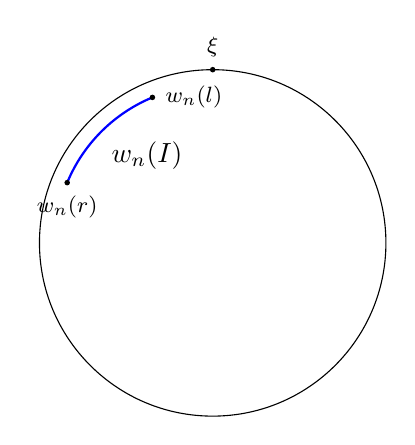
\begin{tikzpicture}[scale=1]
\tikzstyle{vertex} = [shape = circle,fill = black,minimum size = 2pt,inner sep=0pt]

\draw (0,0) circle (2.2);

%\draw[thick,red] ([shift=(22.5:2)]0,0) arc (22.5:90-22.5:2) node[black, below left, pos=.5] {$I_{n,\omega}$};
\draw[thick,blue] ([shift=(180-22.5:2)]0,0) arc (180-22.5:90+22.5:2) node[black, below right, pos=.5] {$w_n(I)$};

\node[vertex, label={[font=\footnotesize] above:$\xi$}] (0) at (0,2.2) {};

\node[vertex, label={[font=\footnotesize] below:$w_n(r)$}] (0) at ([shift=(180-22.5:2)]0,0) {};

\node[vertex, label={[font=\footnotesize] right:$w_n(l)$}] (0) at ([shift=(90+22.5:2)]0,0) {};

\end{tikzpicture}\hfill
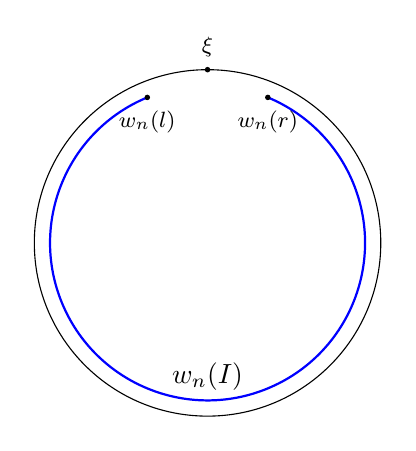
\begin{tikzpicture}[scale=1]
\tikzstyle{vertex} = [shape = circle,fill = black,minimum size = 2pt,inner sep=0pt]

\draw (0,0) circle (2.2);

%\draw[thick,red] ([shift=(22.5:2)]0,0) arc (22.5:90-22.5:2) node[black, below left, pos=.5] {$I_{n,\omega}$};
\draw[thick,blue] ([shift=(90+22.5:2)]0,0) arc (90+22.5:450-22.5:2) node[black, above, pos=.5] {$w_n(I)$};

\node[vertex, label={[font=\footnotesize] above:$\xi$}] (0) at (0,2.2) {};

\node[vertex, label={[font=\footnotesize] below:$w_n(l)$}] (0) at ([shift=(90+22.5:2)]0,0) {};

\node[vertex, label={[font=\footnotesize] below:$w_n(r)$}] (0) at ([shift=(450-22.5:2)]0,0) {};

\end{tikzpicture}\hfill
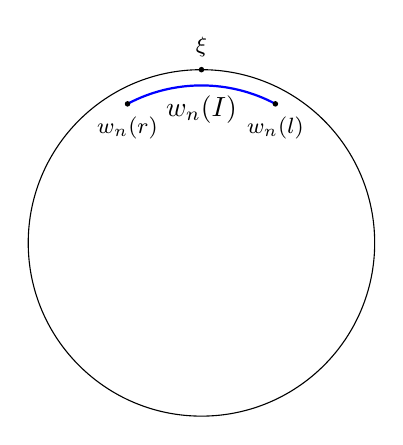
\begin{tikzpicture}[scale=1]
\tikzstyle{vertex} = [shape = circle,fill = black,minimum size = 2pt,inner sep=0pt]

\draw (0,0) circle (2.2);

%\draw[thick,red] ([shift=(22.5:2)]0,0) arc (22.5:90-22.5:2) node[black, below left, pos=.5] {$I_{n,\omega}$};
\draw[thick,blue] ([shift=(90-28:2)]0,0) arc (90-28:90+28:2) node[black, below, pos=.5] {$w_n(I)$};

\node[vertex, label={[font=\footnotesize] above:$\xi$}] (0) at (0,2.2) {};

\node[vertex, label={[font=\footnotesize] below:$w_n(r)$}] (0) at ([shift=(90+28:2)]0,0) {};

\node[vertex, label={[font=\footnotesize] below:$w_n(l)$}] (0) at ([shift=(90-28:2)]0,0) {};

\end{tikzpicture}
    \caption{The interval $I$ and the boundary point $\xi$ (left), and the interval $w_n(I)$ and $\xi$ when $n$ is of type I, II and III (center, right and below respectively).}
    \label{fig:types}
\end{figure}

\begin{proposition}\label{prop:typeIII}
    For $\nu$-almost every $\xi \in S^1 \setminus I$ and every $\eta \in (\nu(I),1)$ there exists $N \in \N$ such that
    \[
    \frac{1}{n}\E^\xi \left[\, \abs{0 \leq k \leq n \mid k \emph{ is of type III} } \,\right] \leq \eta
    \]
for all $n \geq N$.
\end{proposition}
\begin{proof}
    The statement follows from the equality
    \[
    \E^\xi\left[\, \abs{0 \leq k \leq n \mid k\text{ is of type III}}\,\right] = \sum_{k = 0}^n \P^\xi\left[ w_n^{-1}(\xi) \in I\right]
    \]and the equidistribution of $\{w_n^{-1}(\xi)\}_{n \in \N}$ from Proposition \ref{prop:equidistributionXi}.
\end{proof}

 \subsection{Finding good collections, II} 
Consider the space $(S^1, \nu)$ where $\nu$ is the unique $\mu$-stationary probability measure on $S^1$.
From now on, fix an element $a \in T \setminus \{e_T\}$ and a closed interval $I \subset S^1$ such that $\mathrm{supp}(a) \subseteq I$ and $\nu(I) < 1$.

\begin{comment}
  \begin{thm}[CURRENTLY INCOMPLETE!]
For every $n \in \N$, define the random variable $Z_n \in \N$ as the maximal number of mutually disjoint intervals in $\{I, w_1^{-1}(I), \cdots, w_n^{-1}(I)\}$.
Then $\liminf_{n \to \infty} \E^\xi[Z_n]/n$ is positive.
\end{thm}
\begin{proof}
Define $C_j$ as the event that $w_j^{-1}(I)$ is disjoint from $w_i^{-1}(I)$ for all $1 \leq i \leq j-1$. 
Notice that
\[
\E^\xi[Z_n] \geq \E^\xi \left[ \sum_{j = 1}^n 1_{C_j}\right]
\] since a greedy strategy for finding a maximal subset of disjoint intervals is to include $w_j^{-1}(I)$ at time $j$ if it is disjoint from all the $w_i^{-1}(I),\, 1 \leq i \leq j-1$. We have
\begin{align*}
\E^\xi\left[ \sum_{j = 1}^n 1_{C_j}\right] &= \sum_{j = 1}^n \P^\xi\left[ w_j^{-1}(I) \cap w_i^{-1}(I) = \emptyset \text{ for all }1 \leq i \leq j-1 \right]\\
&=\sum_{j = 1}^n\P^\xi\left[ g_1^{-1} \cdots g_j^{-1}(I) \cap g_1^{-1} \cdots g_i^{-1}(I) = \emptyset \text{ for all }1 \leq i \leq j-1 \right] \\
%&=\sum_{j = 1}^n\P^\xi\left( g_{i+1}^{-1} \cdots g_j^{-1}(I) \cap I = \emptyset \text{ for all }1 \leq i \leq j-1 \right) \\
%&=\sum_{j = 1}^n\P^\xi\left( g_{j-i}^{-1} \cdots g_1^{-1}(I) \cap I = \emptyset \text{ for all }1 \leq i \leq j-1 \right)
& = \sum_{j = 1}^n\P^\xi\left[ g_{j}\cdots g_{i+1}(I) \cap I = \emptyset \text{ for all }1 \leq i \leq j-1 \right]\\
&= \sum_{j = 1}^n\P^\xi\left[ g_1 \cdots g_{j-i}(I) \cap I = \emptyset \text{ for all }1 \leq i \leq j-1 \right],
\end{align*}
where in the last equality we have used that the process $\mathbf{w} = \{w_n\}_{n \in \N}$ conditioned to $\xi(\mathbf{w}) = \xi$ is a time-homogeneous Markov chain in order to justify that $(g_1,\ldots, g_j)$ has the same distribution than $(g_j,\ldots, g_1)$. \textcolor{blue}{This is a lie XD}

Thus $\E\left[\sum_{j = 1}^n 1_{C_j}\right] /n$ converges to $\P^\xi\left[ g_1\cdots g_n(I) \cap I = \emptyset \text{ for all }n \geq 1 \right]$. This quantity is positive: indeed, $\P^\xi$-almost surely we have $\lim_{n \to \infty} d(g_1\cdots g_n(I) , \xi) = 0$, so there exists a $k \in \N$ such that $\P^\xi\left[ g_1 \cdots g_n(I) \cap I = \emptyset \text{ for all }n \geq k \right]$ is positive.% The Markov property shows that $\P^\xi(g_1\cdots g_n(I) \cap I = \emptyset \text{ for all }n \geq 1)$ is also positive. This finishes the proof. 
%\[
%\P\left(g_{j+1}^{-1} \cdots g_n^{-1}(I) \cap I = \emptyset \text{ for all }1 \leq j \leq n-1 \right)
%\]
%and
%\[
%\P\left( w_n^{-1}(I) \cap w_j^{-1}(I) = \emptyset \text{ for all }1 \leq j \leq n-1 \right) = \P\left(
%\]
%Notice that a lower bound for $Z_n$ can be achieved greedily as follows: given a realization of the random walk $\{w_n\}_{n \ge 0}$ define sets of intervals $\cI_n, \, n \in \N$ by setting $\I_0 = \{I\}$, and given $\cI_{n-1}$ define $\c$
\end{proof}  

%Even though the above proof does not hold, it allows us to prove a weaker version. (This is a non-relitivized version: we completely ignore the limit point!) This version is sufficient for our purposes.

\begin{thm}[Lots of disjoint intervals - nonrelativized bound]
.\\As above, let $I$ be a proper interval of $\mathbb{S}^1$.
For every $n \in \N$, define the random variable $Z_n \in \N$ as the maximal number of mutually disjoint intervals in $\{I, w_1^{-1}(I), \cdots, w_n^{-1}(I)\}$.

\textbf{Then} for any $s \in \N$ and sufficiently large $N \in \N$ we have
\[\E[Z_N] \ge \dfrac{N}{2s} \P\left[ w_{is}(I) \cap I = \emptyset \emph{ for all } i \in \N \right]. \]
\end{thm}

Just for the sake of naming things, let us call $\P(w_{is}(I) \cap I = \emptyset \;for\;all\;i \in \N)$ the \textbf{probability of never intersecting} with \textbf{sparsity parameter} $s$.

\begin{proof}
We greedily choose points along the arithmetic progression $\{0,s,2s,3s,4s,...\} \subset \N$.
Without loss of generality let $N = ns$ for some $n \in \N$.
For each $j=1,...,n$ define the event 
\[C_j = \{w_{is}(I)\cap w_{js}(I) = \emptyset  \text{ for all }i=1,...,j-1\}.\]
By greedy choice and the reversibility of the random walk we have
\[\E[Z_N] \geq \sum_{j=1}^n \P[C_j] = \sum_{j=1}^n \P\left[ w_{is}(I) \cap I = \emptyset \text{ for all }i=1,...,j-1\right]. \]
Since the events $\{w_{is}(I) \cap I = \emptyset \text{ for all }i=1,...,j-1\}$ are nested in $j$ we obtain 
\[ \P\left[ w_{is}(I) \cap I = \emptyset \text{ for all }i=1,...,j-1\right]  \xrightarrow[j \to \infty]{} \P\left[ w_{is}(I) \cap I = \emptyset \text{ for all }i \in \N\right],\]
and for the Cesaro averages we conclude that 
\[\dfrac{s}{N} \sum_{j=1}^n \P\left[ w_{is}(I) \cap I = \emptyset \text{ for all }i=1,...,j\right] \xrightarrow[n \to \infty]{} \P\left[ w_{is}(I) \cap I = \emptyset \text{ for all }i \in \N\right]. \]
The result follows for sufficiently large $N$.
\end{proof}

\begin{proposition}[Lower bound on the probability of never intersecting]
    .\\\textbf{Assume} that there exists $\lambda>0$ such that for all $n \in \N$
    \[\sup_{y \in \mathbb{S}^1} \E \left[  d(w_n y, \xi) \right] \leq e^{-\lambda n}.\]
    
    \textbf{Then} there exists a sparsity $s \in \N$ and $\Xi \subseteq \mathbb{S}\setminus I$ of measure $\nu(\Xi) \ge (1-\nu(I))/2$ such that
    \[ \P\left[ w_{is}(I) \cap I = \emptyset \emph{ for all }i \in \N \mid \xi \in \Xi\right]  > 4/5.\]
    As a consequence, we have that
    \[\E [Z_N] \geq \frac{N}{2s} \nu(\Xi) \P\left[ w_{is}(I) \cap I = \emptyset \emph{ for all }i \in \N \mid \xi \in \Xi\right] \doteq \Omega_{\lambda, I, \nu}(N).\]
\end{proposition}
%Note that if we knew the probability density of $\nu$ then we could make the sparsity constant $s$ in the above proposition effective.
\begin{proof}
    Since $\nu$ is continuous we have
    \[\nu(\{\xi \mid  d(\xi,I)<\epsilon\}) \xrightarrow[\epsilon \to 0]{} 0,\]
    so there exists $\epsilon>0$ such that
    \[\Xi \doteq \{\xi \mid  d(\xi,I)>\epsilon\}\]
    has $\nu$-measure $\geq (1-\nu(I))/2$.
    Now choose a sparsity $s$ such that $e^{-\lambda s/2} < \min\{\epsilon \nu(\Xi)/2, 1/10\}$, and denote the endpoints of the interval by $I = [l,r]$.
    For each $i \in \N$ we use the assumption and the Markov inequality to get
    \begin{align*} \nu(\Xi) \P\left[ w_{is}(I) \cap I \neq \emptyset \mid \xi \in \Xi\right]  
    & \leq \nu(\Xi) \P\left[  \max\{d(w_{is}(l), \xi), d(w_{is}(r), \xi)\} > \epsilon \mid \xi \in \Xi \right] \\ & = \P\left[ \max\{d(w_{is}(l), \xi), d(w_{is}(r), \xi)\} > \epsilon\right] 
    \leq e^{-\lambda is}\frac{2}{\epsilon}\end{align*} 
    and hence
    \[ \P\left[ w_{is}(I) \cap I \neq \emptyset \mid \xi \in \Xi \right] 
    \leq 2 e^{-\lambda s/2} e^{-\lambda (i-1)s}.\]
    
    By the union bound we get a geometric series and conclude that
    \[ \P\left[ \text{there exists }i \text{ such that }w_{is}(I) \cap I \neq \emptyset \mid \xi \in \Xi \right] \leq 2 e^{-\lambda s/2} \leq 1/5. \qedhere \]
\end{proof}

\subsection{Good collections are satisfactory}

Consider a collection $(w, i_1, \ldots, i_k)$ where $w = \{x_l\}_{l \in \{1,\ldots, n\}\setminus \{i_1,\ldots, i_k\}}$ and define for all $1 \leq j \leq k$ the elements
\begin{equation}\label{eq:gj}
\tilde{w}_j = x_1x_2 \cdots x_{i_1 - 1} x_{i_1 + 1} \cdots x_{i_j-1}
\end{equation}
and 
\[
\tilde{g}_j = x_{i_{j-1}+ 1} \cdots x_{i_j - 1}, 
\]so $\tilde{w}_j = \tilde{g}_1\cdots \tilde{g}_j$. 
The product in \eqref{eq:gj} is taken over the indices $l  \in \{1,\ldots, n\}\setminus \{i_1,\ldots, i_k\},\, l < i_j$. By definition, we set $i_0 = 0$.

We say that $(w, i_1, \ldots, i_k)$ is \emph{good} if the intervals $I, \tilde{w}_1(I),\ldots, \tilde{w}_k(I)$ are pairwise disjoint.
\begin{proposition}
    Let $q$ be a good collection. Then $T^{a, e_T}(q)$ is satisfactory.
\end{proposition}
\begin{proof}
    Write $q = (w, i_1, \ldots, i_k)$ and $\tilde{g_1},\ldots, \tilde{g_k},\, \tilde{w_1},\ldots, \tilde{w_k}$ %\, w = \{x_k\}_{l \in \{1,\ldots, n\} \setminus \{i_1,\ldots, i_k\}}$ and $g_1,\ldots, g_k$ 
    as in the definition of a good collection. Consider two distinct trajectories $\mathbf{f}, \mathbf{h} \in T^{a,e_T}(q)$ and let $1\leq j \leq k$ be the largest index such that the increments at time $i_j$ in $\mathbf{f}$ and $\mathbf{h}$ are different. We may assume that this increment is $a$ in $\mathbf{f}$ and $e_G$ in $\mathbf{h}$. Write
    \[
    f_n = \tilde{g}_1 a_1 \tilde{g}_2 a_2 \cdots a_{j-1}\tilde{g}_j a u \quad \text{ and } \quad h_n = \tilde{g}_1 b_1\tilde{g}_2 b_2 \cdots b_{j-1} \tilde{g}_j u
    \]where the $a_k, b_k$ are in $\{a, e_G\}$ for all $k = 1,\ldots, j-1$. 
    
    We claim that
    \[
    \restr{(\tilde{g}_1 a_1 \cdots a_{j-1}\tilde{g}_j)}{I} = \restr{(\tilde{g}_1b_1  \cdots b_{j-1}\tilde{g}_j)}{I}.
    \] Indeed, first notice that since the intervals \[
    \tilde{w}_{j-1}(I), \tilde{w}_{j-2}(I),\ldots, \tilde{w}_1(I)
    \]are disjoint from $\tilde{w}_j(I)$, it follows that the intervals
    \[
    \tilde{g}_j^{-1}(I), (\tilde{g}_{j-1}\tilde{g}_j)^{-1}(I),\ldots, (\tilde{g}_2\cdots \tilde{g}_j)^{-1}(I)
    \]are all disjoint from $I$. Now
    \[
    \restr{(a_{j-1}\tilde{g}_j)}{I} = \restr{(b_{j-1}\tilde{g}_j)}{I}
    \] since $\tilde{g}_j^{-1}(I)$ is disjoint from $I$. In the same way, we see inductively that for all $k = j, j-1,\ldots, 1$, the equality
    \[
     \restr{(a_k \tilde{g}_{k+1} \cdots a_{j-1}\tilde{g}_j)}{I} = \restr{(b_k \tilde{g}_{k+1}\cdots b_{j-1}\tilde{g}_j)}{I}
    \]follows from the fact that $(\tilde{g}_k \cdots \tilde{g}_j)^{-1}(I)$ is disjoint from $I$. This proves the claim.
    
    %this follows from the fact that the intervals
    %\[
    %\tilde{g}_j^{-1}(I), (\tilde{g}_{j-1}\tilde{g}_j)^{-1}(I),\ldots, (\tilde{g}_2\cdots \tilde{g}_j)^{-1}(I)
    %\]are all disjoint from $I$, and in turn, these intervals are disjoint since the
    %\[
    %\tilde{w}_{j-1}(I), \tilde{w}_{j-2}(I),\ldots, \tilde{w}_1(I)
    %\]are disjoint from $\tilde{w}_j(I)$.

    Thus $f_n$ differs from $h_n$ on $u^{-1}(I)$, and we conclude that $T^{a, e_T}(q)$ is satisfactory.
    %The intervals where the functions $f_nu^{-1}$ and $g_n u^{-1}$ may differ are the intervals
    %\[
   % 
   % \]
    % By descending induction on $k = j-1 ,\ldots, 1$ we prove that
    %\[
    %f_n g_n^{-1} = w_1 a_1 \cdots a_k w_{k+1} a^{a_k}
    %\]
    %
    %Now
    %\begin{align*}
    %    f_n g_n^{-1} &= w_1 a_1 \cdots a_{j-1}w_j a w_j^{-1} b_{j-1}^{-1}\cdots b_1^{-1} w_1^{-1} \\
   %     & = w_1 a_1 \cdots a_{j-2}w_{j-1}a^{a_{j-1}w_j} (a_{j-1} b_{j-1}^{-1}) w_{j-1}^{-1} \cdots b_1^{-1} w_1^{-1}\\
   %     & = w_1 \cdots a_{j-3}w_{j-2} a^{a_{j-2} w_{j-1} a_{j-1}w_j}(a_{j-1}b^{-1}_{j-1})^w_{j-1} \cdots b_1^{-1} w_1^{-1}
   % \end{align*}
    %and let $1 \leq j \leq k$ be the first index such that $f_{i_j}$ and $h_{i_j}$ differ.
    %Consider two elements $f_1, f_2 \in T$ that arise as the time $n$ elements of two distinct trajectories $\mathbf{f}_1, \mathbf{f}_2 \in T^{a,e_T}(q)$. Let $1 \leq j \leq k$ be the first moment such that $\mathbf{f}_1$ and $\mathbf{f}_2$ differ.
   % Write \[f_n = u a_j w_j a_{j+1} w_{j+1} \cdots a_n w_n \quad \text{and} \quad h_n = u a_j' w_j a_{j+1}' w_{j+1} \cdots a_n' w_n\] where the $a_k, a_k', \, k = j,\ldots, n$ are in $\{a,e_G\}$ and $w_k = x_{i_k + 1} \cdots x_{i_{k+1}-1}$ for $k = j,\ldots, n$. The functions $f_n$ and $h_n$ differ in the interval 
\end{proof}

\subsection{Putting everything together}

Let's put everything together to get the result (that the Poisson boundary is NOT the circle).
\\1.We fix $I$ and $a$ and for every sparsity $s$ obtain a lower bound on $\E [Z_n]$ in terms of the probability of never intersecting.
\\2. We are given $\nu$, so we choose the sparsity $s$ appropriately and get a lower bound for some $0 < c < 1$:
$$\E_\xi \E^{\xi} Z_n \ge c n.$$
\\3. For each $\xi \in \mathbb{S}^1$ and each $n$, by pigeonhole we get a set of good collections $A_{n,\xi}$ which satisfy
$$\frac{k(q)}{n} \geq \frac{\E^{\xi} Z_n}{2n}$$
such that
$$\P^\xi(\cup_{q \in A_{n,\xi}} T^{a,e_G}(q))\geq \frac{\E^{\xi} Z_n}{2n}.$$
When $\xi \in I$ we should expect $k(q)$ to be bounded in $n$, but that is OK.
What we really care about is the growth of $k(q)$ for an average $\xi$, and we know that the expectation must grow linearly.

Each of these collections are satisfactory by the above section and they are also disjoint (\textbf{TODO}: give a precise definition of $A_{n,\xi}$).
\\4. We now follow Erschler's entropy estimate:
\begin{proof}
The proof is essentially the same as before.
Let $\nu$ be the conditional measure of $\mu$ on the set $\{e_G,a\}$.
Now $a$ is $\mathbb{S}^1-I$-stable, and the times $i_1,...,i_k$ of $q$ are those which make the images under $I$ form disjoint partitions.
It follows that for every $q\in A_n$ and every $\xi\in \mathbb{S}^1-I$, 
the normalized restriction of $\P^{\xi}$ restricted to $T^{a,e_G}(q)$ is the product measure $\nu^k$, so
\[
H^\xi(w_n \mid T^{a, e_G}(q)) = H(\nu^k) = k(q) H(\nu).
\] 
Thus 
	\begin{align*}
		\E_{\xi} H^{\xi}(w_n)& \ge \E_{\xi} \left(\sum_{q\in A_{n,\xi}}H^{\xi}(w_n\mid T^{a,e_G}(q))\P^{\xi}(T^{a,e_G}(q))\right) & \\
        & \ge \E_{\xi} \left((\min_{q \in A_{n,\xi}} k(q))\; H(\nu) \sum_{q\in A_n}\P^{\xi}(T^{a,e_G}(q))\right) & \\
        & \ge \E_{\xi} \left(\E^{\xi} \frac{Z_n}{2}\; H(\nu) \E^{\xi} \frac{Z_n}{2n}\right) & \\
        & \ge \dfrac{H(\nu)}{4n}\E_{\xi} (\E^{\xi} Z_n)^2 \ge \dfrac{H(\nu) c^2 n}{4}
	\end{align*}
where we used Jensen at the last step.
So for every $n\ge 1$ we have
\[
\frac{H(w_n|\xi)}{n} = \frac{\E_{\xi} H^{\xi}(w_n)}{n}\ge \dfrac{H(\nu) c^2}{4}.
\]

Note that by sub-additivity of entropy and the fact the entropy reduces when conditioning, it follows that for all $\xi$ and all $n$, $\frac{H^{\xi}(w_n)}{n} \leq H(\mu)$.
By applying Fatou's lemma to $H(\mu)-\frac{H^{\xi}(w_n)}{n}$ (or by the DCT) we get
\[
\E_{\xi} h^{\xi}(\mu) = \E_{\xi} \limsup_n \frac{H^{\xi}(w_n)}{n} \ge \limsup_n \E_{\xi} \frac{H^{\xi}(w_n)}{n}\ge \dfrac{H(\nu) c^2}{4}>0.
\]
This means that $h^{\xi}(\mu) >0$ for a set of positive measure of $\xi$'s.    
\end{proof}
\textbf{All that remains to be shown:}
there exists $\lambda>0$ such that for all $n \in \N$
    $$\sup_{y \in \mathbb{S}^1} \E d(w_n y, \xi) \leq e^{-\lambda n}.$$
(Note: the expectation is NOT conditional on the boundary point. This is much weaker from the original assumption i had in mind.)
Q: Is this covered by Lemma 4.6?

Martín: YES! It's a lot easier to prove than the nonrelativized version. There's still a thing I haven't figured out about the optimal moment assumptions, but with the moment assumptions written at the beginning of subsection 4.2 I'm absolutely sure it works.
\end{comment}